\documentclass[12pt,aspectratio=169]{beamer}
\usepackage[utf8]{inputenc}
\usepackage[T1]{fontenc}
\usepackage[french]{babel}
\usepackage{lmodern,amsmath,amssymb,booktabs}
\usetheme{Madrid}
\setbeamertemplate{navigation symbols}{}
\setbeamertemplate{footline}[frame number]
\setbeamertemplate{itemize items}[circle]
\title{Maillages et précision de la méthode des éléments finis}
\subtitle{Une onde acoustique harmonique : géométrie, convergence et pollution numérique}
\author{Yann MOUSSU}
\institute{CentraleSupélec}
\date{10 octobre 2026}
\newcommand{\figureresultat}[2]{\begin{center}\includegraphics[width=#2\textwidth,height=.53\textheight,keepaspectratio]{../report/figures/#1}\end{center}}
\begin{document}
\begin{frame}\titlepage\end{frame}

\begin{frame}{Préambule}
Le projet relie la qualité géométrique du maillage à la précision d'une approximation triangulaire $P_1$ de l'équation de Helmholtz.
\begin{block}{Démarche}
Construire et contrôler le maillage, résoudre un problème dont la solution exacte est connue, puis mesurer l'erreur lorsque la résolution et le nombre d'onde varient.
\end{block}
\begin{enumerate}
\item \textbf{Maillage :} aires, critères de qualité, déplacement et opérations géométriques.
\item \textbf{Méthode des éléments finis :} formulation, normes d'erreur, convergence sur maillages réguliers et déplacés.
\end{enumerate}
Les résultats distinguent les tendances mesurées des propriétés théoriques d'interpolation et de stabilité.
\end{frame}

\section{Maillage}
\begin{frame}{Représentation et contrôle du maillage}
Le maillage est décrit par les coordonnées des nœuds, une connectivité aplatie et un tableau de pseudo-pointeurs.
\[
\mathrm{l2g}(e,i)=\texttt{elem2nodes}[p_e+i],\qquad
p_{e+1}-p_e\in\{3,4\}.
\]
\begin{itemize}
\item Les sommets d'un élément sont ordonnés le long de son contour.
\item Les indices, les coordonnées finies et les incidences des arêtes sont vérifiés.
\item Les cellules dégénérées, les quadrangles croisés et les orientations incompatibles sont refusés.
\end{itemize}
\begin{block}{Rôle des contrôles}
Une aire positive est nécessaire au calcul ; elle ne suffit pas à garantir une bonne forme ni à détecter tout recouvrement arbitraire.
\end{block}
\end{frame}

\begin{frame}{Alternatives géométriques et leurs limites}
Plusieurs solutions simples sont correctes dans un cadre restreint, mais ne conviennent pas à toute la famille de maillages.
\begin{itemize}
\item Pour Q1, l'aire absolue ne distingue pas deux orientations opposées : le signe est contrôlé séparément.
\item Pour Q4, un déplacement absolu fixe devient deux fois plus fort relativement à $h$ à chaque raffinement ; on retient $\mu\ell_j$.
\item Pour Q7, le trapèze $(0,0),(2,0),(1,1),(0,1)$ donne une moyenne des sommets $(3/4,1/2)$, différente du centroïde $(7/9,4/9)$.
\end{itemize}
Ces exemples motivent les contrôles et les constructions détaillés ensuite. Une direction aléatoire fixée ou une autre diagonale restent des alternatives valables.
\end{frame}
\begin{frame}{Aires et critères de qualité}
Les questions Q1 à Q3 portent sur l'aire et les deux critères géométriques du cours. Pour un triangle :
\[
a_T=\frac12\det(P_1-P_0,P_2-P_0),\quad |T|=|a_T|,\quad
\rho_T=\frac{|T|}{(\ell_1+\ell_2+\ell_3)/2}.
\]
\[
Q_T=\frac{\sqrt3}{6}\frac{h_{\max,T}}{\rho_T},\qquad
E_T=\frac{\min(\ell_1,\ell_2,\ell_3)}{(\ell_1+\ell_2+\ell_3)/3}.
\]
\begin{itemize}
\item L'aire signée distingue inversion et dégénérescence.
\item Pour l'équilatéral, $Q_T=E_T=1$ ; $Q_T$ augmente lorsque la forme se dégrade.
\item Le terme \emph{medium} est interprété comme la moyenne arithmétique des longueurs, convention conservée dans tous les résultats.
\end{itemize}
\end{frame}

\begin{frame}{Déplacement des nœuds et frontière fixe}
Pour Q4, la longueur locale est calculée à partir des éléments incidents au nœud $j$ :
\[
\ell_j=\frac{1}{\#\mathcal E(j)}\sum_{e\in\mathcal E(j)}\bar\ell_e,
\qquad P'_j=P_j+\mu\ell_j\frac{d}{\|d\|}.
\]
Pour Q5, cette règle s'applique uniquement aux nœuds internes.
\begin{itemize}
\item Une arête appartient au bord si elle possède un seul élément incident.
\item Les coordonnées des nœuds du bord restent exactement inchangées.
\item Les études utilisent $d=(1,0)$ et $\mu=0,1$ ; aucune perturbation aléatoire n'est introduite.
\end{itemize}
\begin{block}{Validité géométrique}
Les signes des aires sont contrôlés après déplacement. Une amplitude qui inverse ou dégénère un élément est refusée.
\end{block}
\end{frame}

\begin{frame}{Comparaison avant et après déplacement}
Pour Q6, on compare 1365 nœuds et 2560 triangles sur une frontière fractale de niveau 3, dont la construction sera précisée pour Q10. Le déplacement interne conserve le contour.
\begin{center}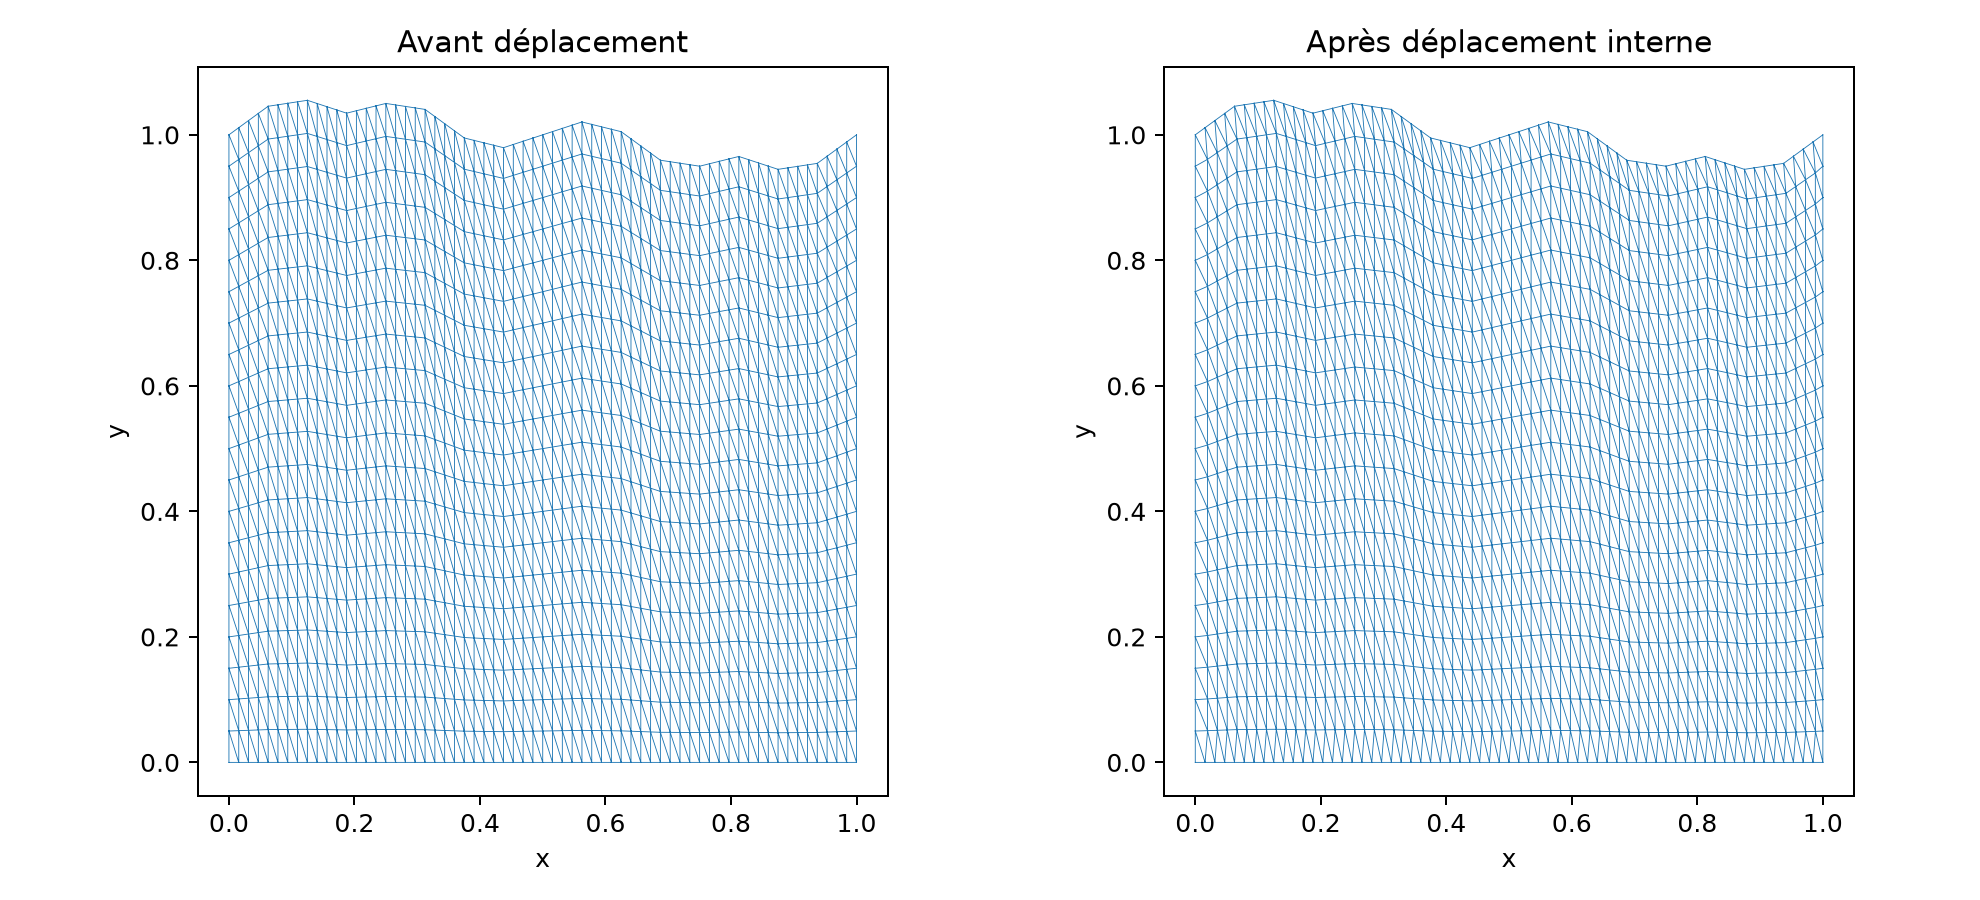
\includegraphics[width=.95\textwidth,height=.50\textheight,keepaspectratio]{../report/figures/mesh_comparison.png}\end{center}
L'aire totale reste égale à 1 ; l'aire minimale passe de $3,6914\times10^{-4}$ à $2,9031\times10^{-4}$, sans inversion.
\end{frame}

\begin{frame}{Interprétation des indicateurs géométriques}
La comparaison de Q6 montre une dégradation locale de la forme. Les histogrammes utilisent les mêmes classes avant et après déplacement.
\begin{columns}[c]
\begin{column}{.53\textwidth}
\small
\begin{tabular}{lrr}\toprule
Indicateur & Avant & Après \\\midrule
Aspect maximal & 3,1506 & 3,4639 \\
Facteur d'arête minimal & 0,3767 & 0,3134 \\
Angle minimal & $13,97^\circ$ & $12,77^\circ$ \\\bottomrule
\end{tabular}

\medskip
Le déplacement conserve la validité du maillage, mais ne constitue pas un algorithme d'amélioration de sa qualité.
\end{column}
\begin{column}{.46\textwidth}
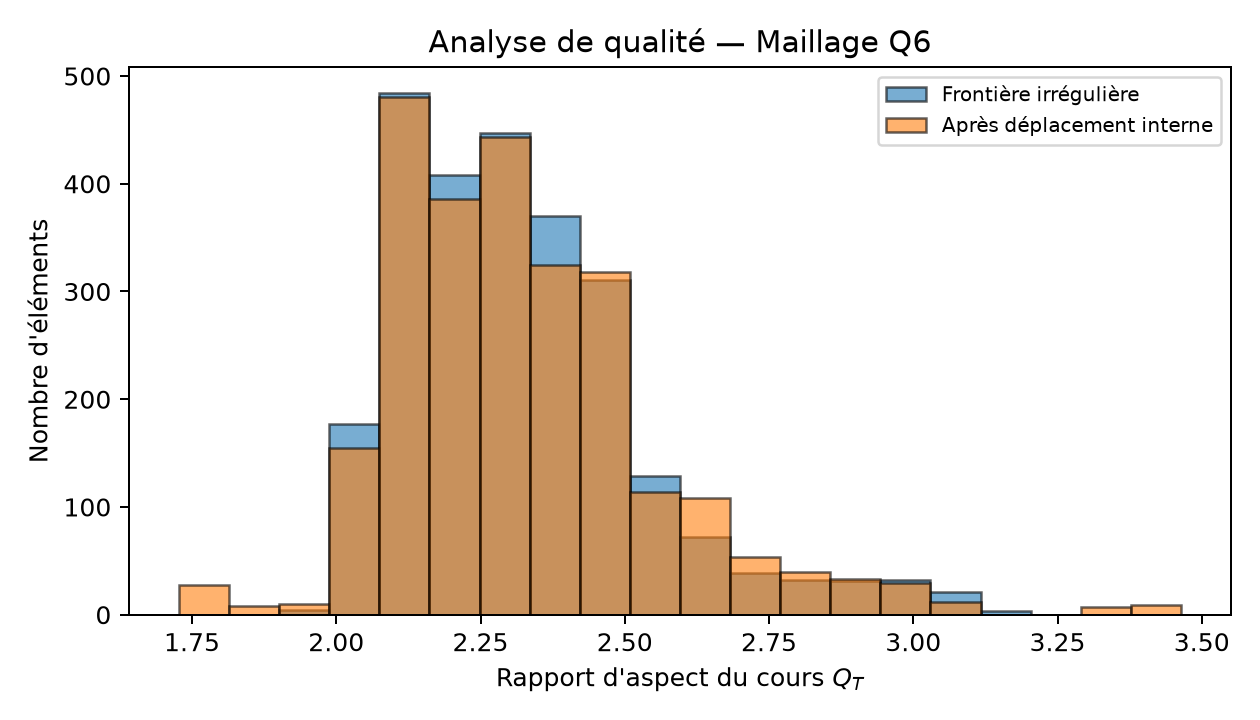
\includegraphics[width=\textwidth]{../report/figures/Figure2.png}
\end{column}
\end{columns}
\end{frame}

\begin{frame}{Barycentre, subdivision et opérations topologiques}
Les questions Q7 à Q9 complètent les outils de manipulation du maillage.
\begin{itemize}
\item \textbf{Q7 :} centroïde surfacique ; pour un triangle, $G=(P_0+P_1+P_2)/3$.
\item \textbf{Q8 :} découpage des quadrangles par une diagonale admissible ; orientations et somme des aires conservées.
\item \textbf{Q9(i)--(ii) :} ajout ou suppression d'un élément, avec reconstruction de la connectivité et des pseudo-pointeurs.
\item \textbf{Q9(iii)--(iv) :} ajout d'un nœud isolé ; suppression seulement s'il n'est plus référencé, puis renumérotation des indices suivants.
\end{itemize}
\begin{block}{Portée des opérations}
Les triangles des maillages mixtes sont conservés. Les opérations topologiques modifient les tableaux, sans retriangulation automatique du domaine.
\end{block}
\end{frame}

\begin{frame}{Construction d'une frontière fractale}
Pour Q10, le motif polygonal $g$ passe par les hauteurs $0,1,0,-1,0$ aux abscisses $0,1/4,1/2,3/4,1$ et est prolongé périodiquement.
\[
d_L(x)=0,05\sum_{j=0}^{L-1}0,6^j g(2^jx),\qquad d_0=0.
\]
\begin{itemize}
\item Chaque niveau ajoute le motif à une échelle horizontale divisée par deux et verticale multipliée par 0,6.
\item La série limite converge ; les pentes aux petites échelles croissent comme $\sum_j1,2^j$. Les niveaux finis sont ses approximations polygonales.
\item Le niveau est indépendant de la résolution ; $n_x$ doit être multiple de $2^{L+1}$ pour représenter tous les sommets.
\end{itemize}
La hauteur reste positive puisque $|d_L|\leq0,125<1$.
\end{frame}

\begin{frame}{Niveaux fractals et conservation de l'aire}
L'antisymétrie $d_L(1-x)=-d_L(x)$ annule la somme trapézoïdale du relief. L'aire reste égale à 1 à chaque niveau.
\begin{center}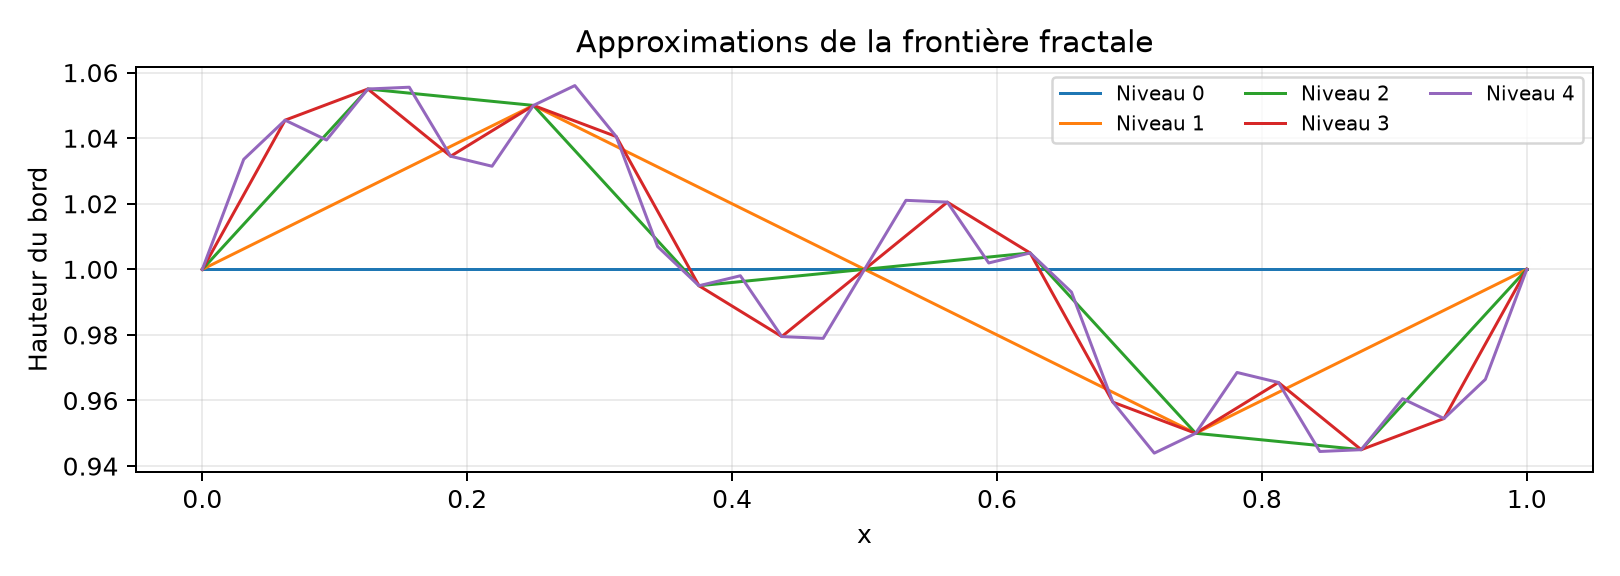
\includegraphics[width=.9\textwidth,height=.43\textheight,keepaspectratio]{../report/figures/fractal_levels.png}\end{center}
La transformation $y(x,\eta)=\eta(1+d_L(x))$ répartit la déformation sur toutes les rangées. Les niveaux 0 à 4 sont contrôlés sur $64\times20$ : aire conservée et triangles positifs.
\end{frame}

\begin{frame}{Extraction du sous-maillage de frontière}
La question facultative Q11 utilise les arêtes d'incidence 1 pour construire un maillage local composé de segments.
\[
P^\Gamma_j=P_{\mathrm{l2g}_\Gamma(j)}.
\]
\begin{itemize}
\item Les coordonnées et la connectivité sont exprimées dans la numérotation locale du bord.
\item Les pseudo-pointeurs augmentent de 2 pour chaque segment.
\item La correspondance $\mathrm{l2g}_\Gamma$ et l'élément volumique adjacent sont conservés.
\end{itemize}
\begin{block}{Vérification}
Sur le maillage $64\times20$, le bord comporte 168 nœuds et 168 segments. Les indices locaux et leur correspondance vers les coordonnées globales sont contrôlés.
\end{block}
\end{frame}


\section{Méthode des éléments finis}
\begin{frame}{Modèle acoustique et solution exacte}
La convention harmonique est $\widetilde p(x,t)=\operatorname{Re}(u(x)e^{-\mathrm{i}\omega t})$, avec $k=\omega/c$. Sur $\Omega=(0,1)^2$ :
\[
-\Delta u-k^2u=0\quad\text{dans }\Omega,\qquad
u=e^{\mathrm{i}kx}\quad\text{sur }\partial\Omega.
\]
La solution exacte $u^*(x,y)=e^{\mathrm{i}kx}$ permet une mesure directe de l'erreur.
\begin{itemize}
\item Milieu homogène sans amortissement ; propagation suivant $x$.
\item $k=\pi,2\pi,3\pi$, hors du spectre continu $\pi^2(m^2+n^2)$, $m,n\geq1$.
\item La pollution étudiée est l'erreur numérique de propagation ; les amplitudes sont normalisées.
\end{itemize}
\end{frame}

\begin{frame}{Formulation faible et matrices élémentaires}
Avec $v\in H^1_0(\Omega)$, l'identité de Green conduit à
\[
\int_\Omega\nabla u\cdot\nabla v-k^2\int_\Omega uv=\int_\Omega fv.
\]
Les fonctions de base $P_1$ sont affines sur chaque triangle. Leurs gradients sont constants et donnent
\[
(K_T)_{ij}=|T|\nabla\varphi_i\cdot\nabla\varphi_j,\qquad
M_T=\frac{|T|}{12}\begin{pmatrix}2&1&1\\1&2&1\\1&1&2\end{pmatrix}.
\]
\begin{itemize}
\item La formulation bilinéaire suit la convention du cours ; les bases sont réelles.
\item La correspondance locale/globale permet l'assemblage de $K$, $M$ et $F$.
\end{itemize}
\end{frame}

\begin{frame}{Alternatives pour le stockage et la résolution}
\begin{block}{Matrices pleines : résultat de stockage}
Sur $128\times32$, stocker $K,M$ en plein demanderait $276,52$ Mio. Ce coût théorique inclut les coefficients nuls et croît comme $N^2$.
\end{block}
\begin{block}{Gradient conjugué standard : condition non satisfaite}
Sur $16\times4$ à $k=2\pi$, une direction propre de $A$ est négative et 44 sont positives. La matrice est indéfinie : les garanties du cas défini positif ne s'appliquent pas.
\end{block}
Gauss dense reste correct et une méthode itérative adaptée reste possible. Les limites constatées motivent ici une résolution directe exploitant les matrices creuses.
\end{frame}

\begin{frame}{Assemblage et résolution de Dirichlet}
Pour Q1 et Q2, le stockage COO puis CSR de $K,M$ vaut $0,70$ Mio sur $128\times32$, hors facteurs LU et temporaires.
\[
A=K-k^2M,\qquad A_{II}u_I=F_I-A_{IB}g_B,\qquad u_B=g_B.
\]
\begin{itemize}
\item $I$ désigne les nœuds internes et $B$ les nœuds de bord.
\item $K$ et $M$ sont assemblées une fois par géométrie, puis réutilisées pour les trois nombres d'onde.
\item Le système réduit est résolu par factorisation directe creuse.
\end{itemize}
\begin{block}{Contrôle algébrique}
Les 24 solutions ont un résidu relatif inférieur à $4\times10^{-15}$ et une erreur nodale de Dirichlet nulle. L'erreur étudiée provient principalement de la discrétisation et de la stabilité.
\end{block}
\end{frame}


\begin{frame}{Alternative : mesurer seulement l'erreur nodale}
\begin{block}{Résultat obtenu avec la matrice de masse}
Sur $128\times32$ régulier à $k=3\pi$, $\sqrt{e_{\rm nodes}^*Me_{\rm nodes}}=2,5731\times10^{-3}$.
\end{block}
Cette mesure concerne $I_hu^*-u_h$, plutôt que $u^*-u_h$. Si $u_h=I_hu^*$, elle est nulle malgré une erreur continue non nulle.
\begin{block}{Limite du maximum nodal}
À $k=\pi$ sur le même maillage, le maximum nodal vaut $6,18\times10^{-5}$ ; les points intérieurs ne sont pas examinés.
\end{block}
Ces résultats motivent une intégration de l'erreur continue et un échantillonnage à l'intérieur des triangles.
\end{frame}

\begin{frame}{De la quadrature réduite à la précision retenue}
\begin{block}{Alternative : ordres 2 et 3}
À $k=3\pi$, sur les quatre maillages réguliers, l'ordre 2 donne jusqu'à $0,558\,\%$ d'écart relatif $L^2$ par rapport à l'ordre 8. L'ordre 3 donne jusqu'à $6,58\times10^{-6}$, au-dessus du seuil $10^{-7}$ retenu.
\end{block}
\begin{block}{Méthode retenue : ordre 6, contrôlé à l'ordre 8}
Sur les trois normes et les deux familles de maillages, la variation relative reste inférieure à $3\times10^{-13}$. L'ordre 6 est validé, sans être démontré minimal.
\end{block}
La quadrature permet d'évaluer les intégrales FEM ; l'ordre retenu résulte d'un contrôle de précision, sans hypothèse d'intégration exacte de l'exponentielle.
\end{frame}

\begin{frame}{Normes d'erreur continues}
Pour $e=u^*-u_h$, les normes intègrent l'erreur à l'intérieur des éléments :
\[
\|e\|_{L^2}^2=\sum_T\int_T|e|^2,\qquad
\|e\|_{H^1}^2=\|e\|_{L^2}^2+\sum_T\int_T|\nabla e|^2.
\]
\begin{itemize}
\item Les ordres de quadrature 6 et 8 donnent une variation relative inférieure à $3\times10^{-13}$.
\item La norme $L^\infty$ est estimée sur des grilles barycentriques imbriquées, avec stabilisation à $0,5\,\%$.
\item Le maximum nodal et la norme de $I_hu^*-u_h$ ne remplacent pas les erreurs continues demandées.
\end{itemize}
Résultats retenus sur $128\times32$ : $\|e\|_{L^2}=2,8934\times10^{-3}$ à $k=3\pi$ ; maximum intérieur estimé $1,37\times10^{-4}$ à $k=\pi$.
\end{frame}

\begin{frame}{Stockage et définition de l'erreur}
À $k=3\pi$ sur $128\times32$, la norme nodale issue de $M$ vaut $2,5731\times10^{-3}$, contre $2,8934\times10^{-3}$ pour l'erreur continue, soit ici $11,1\,\%$ de moins.
\begin{center}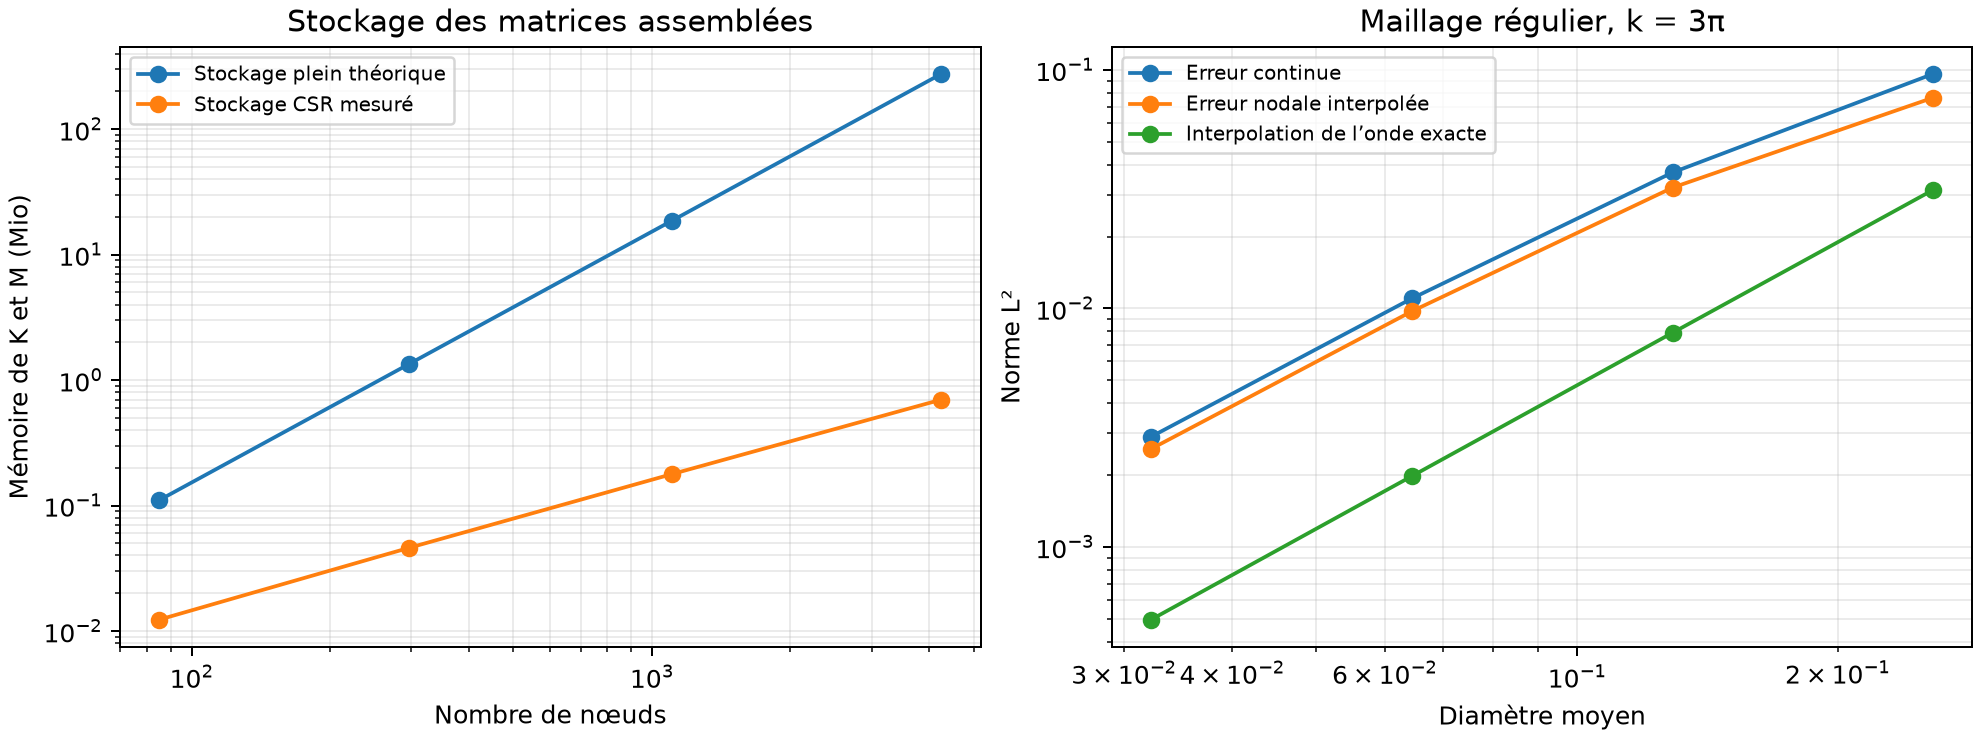
\includegraphics[width=\textwidth,height=.49\textheight,keepaspectratio]{../report/figures/choices.png}\end{center}
Si $u_h=I_hu^*$, l'erreur nodale est nulle, mais l'erreur continue subsiste. Une mesure nodale ne suffit donc pas à évaluer l'erreur demandée.
\end{frame}


\begin{frame}{Protocole et estimation des exposants}
Les deux études utilisent $16\times4$, $32\times8$, $64\times16$ et $128\times32$, pour $k=\pi,2\pi,3\pi$.
\[
\bar h=\frac1{N_e}\sum_T\max_i\ell_{T,i},\qquad
\log(err)\simeq c+\widehat\alpha\log\bar h+\widehat\beta\log k.
\]
\begin{itemize}
\item Les pentes en $h$ sont estimées à $k$ fixé ; celles en $k$ à résolution fixée.
\item L'ajustement conjoint utilise les douze cas de chaque famille.
\item Pour Q2, le déplacement de Q5 de la partie maillage est construit une fois par résolution ; $\bar h$ est ensuite recalculé.
\end{itemize}
Les exposants sont mesurés, sans imposer une loi en $h^2k^3$.
\end{frame}

\begin{frame}{Convergence sur le maillage régulier}
Pour Q1, à $k=\pi$, les pentes globales sont $\alpha_{L^2}=1,9745$ et $\alpha_{H^1}=1,0004$ : les ordres observés sont proches de 2 et de 1.
\figureresultat{Figure5.png}{1}
À $k=3\pi$, la pente locale $L^2$ augmente de 1,3748 à 1,9267 avec le raffinement : le régime asymptotique est approché progressivement.
\end{frame}

\begin{frame}{Sensibilité au nombre d'onde}
Pour Q1, l'erreur augmente avec $k$ à résolution fixée. Cette sensibilité dépend de la norme et de la stabilité du problème.
\figureresultat{Figure6.png}{1}
Les dérivées de l'onde plane portent des puissances de $k$. Trois fréquences permettent une estimation empirique, sans établir un exposant universel.
\end{frame}

\begin{frame}{Modèle conjoint sur le maillage régulier}
Pour Q1, le modèle $L^2$ donne $\widehat\alpha=1,8427$, $\widehat\beta=3,0479$ et $R^2_{\log}=0,99658$, mais un écart relatif maximal proche de $25\,\%$.
\figureresultat{Figure7.png}{1}
En $H^1$, les exposants sont 1,0202 et 2,0454, avec environ $4\,\%$ d'écart maximal : la loi conjointe décrit mieux cette norme sur la grille étudiée.
\end{frame}

\begin{frame}{Convergence après déplacement interne}
Pour Q2, à $k=\pi$, les pentes globales sont $\alpha_{L^2}=2,0730$ et $\alpha_{H^1}=1,0215$. Le bord et les données physiques restent identiques à Q1.
\figureresultat{Figure9.png}{1}
La pente locale $L^2$ diminue de 2,1093 à 2,0319 : les données indiquent une approche de l'ordre 2, sans superconvergence persistante.
\end{frame}

\begin{frame}{Effet du déplacement et quantité combinée}
Pour Q2, le modèle $L^2$ donne $\widehat\alpha=1,9237$ et $\widehat\beta=3,0107$, avec environ $27\,\%$ d'écart relatif maximal.
\figureresultat{Figure12.png}{1}
À $k=\pi$, le déplacement augmente l'erreur $L^2$ d'environ $25\,\%$ sur $16\times4$, contre $1,5\,\%$ sur $128\times32$ : son effet dépend de la résolution.
\end{frame}

\begin{frame}{Interpolation, phase et stabilité}
La décomposition
\[
u^*-u_h=(u^*-I_hu^*)+(I_hu^*-u_h)
\]
éclaire les contributions à l'erreur, dont les normes ne s'additionnent pas exactement.
\begin{itemize}
\item Sur le maillage régulier fin à $k=3\pi$, l'erreur $L^2$ totale vaut $2,893\times10^{-3}$, contre $4,949\times10^{-4}$ pour l'interpolation.
\item Les maxima échantillonnés de phase et d'amplitude atteignent respectivement $3,10\times10^{-3}$ rad et $5,65\times10^{-3}$.
\item La distance $\min_j|\lambda_{h,j}-k^2|$ reste supérieure à 3,17 sur les cas étudiés ; le spectre doit être recontrôlé pour d'autres fréquences.
\end{itemize}
Ces indicateurs étayent l'analyse sans démontrer une domination générale de la dispersion.
\end{frame}

\begin{frame}{Conclusion}
\begin{block}{Maillage}
Les aires, la forme et la frontière sont contrôlées. La construction fractale conserve l'aire à chaque niveau et le déplacement interne conserve exactement le bord.
\end{block}
\begin{block}{Méthode des éléments finis}
Les erreurs continues montrent une convergence proche de l'ordre 2 en $L^2$ et de l'ordre 1 en $H^1$ à $k=\pi$. Le déplacement modifie surtout les erreurs sur les maillages grossiers.
\end{block}
Les ajustements fréquentiels, les écarts au modèle et les diagnostics de phase appellent une interprétation prudente. Une onde suivant $x$, trois fréquences et une direction de déplacement ne suffisent pas à établir une loi universelle de pollution numérique.
\end{frame}
\end{document}
